\documentclass[12pt,a4paper]{article}
\usepackage{fullpage}
\usepackage[top=2cm, bottom=2cm, left=2.5cm, right=2.5cm]{geometry}
\usepackage{amsmath,amsthm,amsfonts,amssymb,amscd}
\usepackage{enumerate}
\usepackage{xcolor}
\usepackage{listings}
\usepackage{graphicx}
\usepackage{caption}
\usepackage{subcaption}

\lstset{
frame = single, 
breaklines=true,
framexleftmargin=1pt}

\title{Program Analysis and Verification:\\Final Project}
\author{Ilya Shervin\\ 308640218 
        \and
        Dmitry Kuznetsov\\ 322081183}


\newcommand{\trans}[1]{[\![\texttt{#1}]\!]}
\newcommand{\atrans}[1]{\trans{#1}^\sharp}
\lstset{basicstyle=\small}
\newcommand{\example}[3]{
\input{#1/examples/example#2.tex}
\begin{figure}[h!]
\centering
\begin{subfigure}{.5\textwidth}
  \centering
  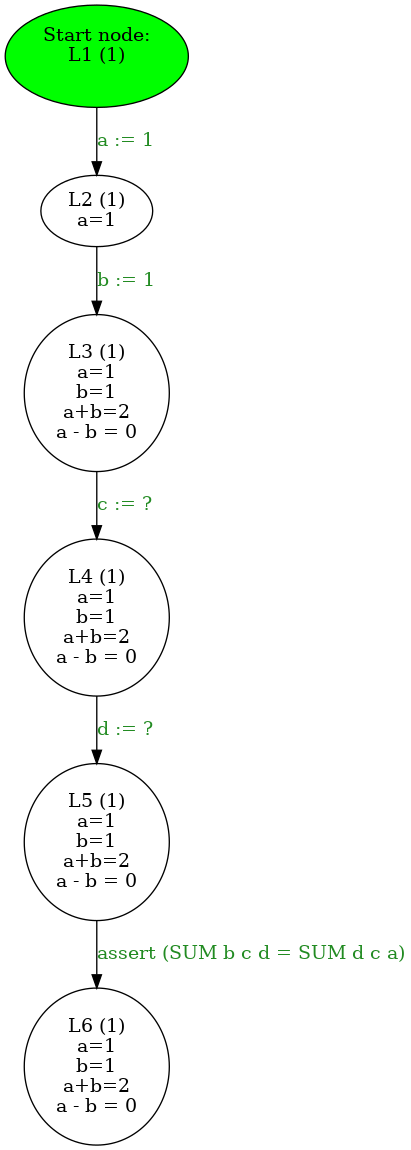
\includegraphics[height=#3\textheight]{./#1/examples/example#2-output/cfg.png}
  \caption{Control flow graph}
\end{subfigure}%
\begin{subfigure}{.5\textwidth}
  \centering
  \lstset{basicstyle=\small}
  \lstinputlisting{#1/examples/example#2.code}
  \caption{Code}
\end{subfigure}
\caption*{\texttt{pipenv run analyze --type #1 docs/#1/examples/example#2.code}}
\end{figure}
}

\newcommand{\parfBasis}[1]{(#1_{even}\leftrightarrow\neg #1_{odd})}

\begin{document}
\maketitle
	\section*{Intro}
	This document accompanies the code of the final project in Program Analysis and Verification class. Following is a brief rundown of code structure and components.
	
	All of the analysis tasks are implemented with Python 3 (3.7+) with the environment and dependencies managed by Pipenv\footnote{https://docs.pipenv.org} (see docs for elaborate usage examples).
	
	Our code relies on the following external software packages:
	\begin{itemize}
		\item SLY\footnote{https://github.com/dabeaz/sly} - a Python implementation of lex/yacc analogues lexers and parsers.
		\item pySMT\footnote{https://github.com/pysmt/pysmt} - a front-end for SAT and SMT solvers
		\item z3-solver\footnote{http://z3prover.github.io} - a back-end for PySMT based on Z3
		\item graphviz\footnote{https://github.com/xflr6/graphviz} - a library for visualization of control flow graphs
		\item sympy\footnote{https://www.sympy.org/} - a library implementing symbolic algebra, used in shape analysis node length computations
		\item pytest\footnote{https://docs.pytest.org} - a test harness
	\end{itemize}
The general method of operation for all of the analysis implementations is as following:
\begin{enumerate}
	\item Parse the input file according to the language definition of the program (parity/sum/shape).
	\item Construct the control flow graph of the program.
	\item Initialize all the nodes in control flow graph to the initial abstract state (depending on the abstract domain of specific analysis).
	\item Perform chaotic iteration until no more updates happen.
	\item Iterate over assert statements and verify their validity against the abstract state of the graph node.
\end{enumerate}
Finally, the results are either printed to the screen as DOT graphs or written to disk as PNG files.

\section*{Installing and Running}
Development of the analysis was done on Linux (any recent Fedora/Ubuntu). To set up a Python environment, run \texttt{pipenv install} in the root directory of the project. This will initialize a new virtual environment and pull required packages. Additionally several system packages are required for execution:
\begin{itemize}
	\item \texttt{graphviz}
	\item \texttt{z3solver}
\end{itemize}

Invocation of analysis is done through \texttt{pipenv run analyze}:
\lstinputlisting{analyze.usage}

The project directory layout is as following:
\begin{itemize}
\item \texttt{analyzeframework/} - Code for basic components used in all analyses (e.g. chaotic iteration, control flow graphs, visualization).
\item \texttt{analyzenumeric/} - Code specific for parity and summation analyses.
\item \texttt{analyzeshape/} - Code specific for shape analysis.
\item \texttt{examples/} - Code examples for all three kinds of included analysis.
\item \texttt{docs/} - Code for building this file.
\item \texttt{analyze.py} - Main entry-point of our program.
\item \texttt{tests/} - Automatic tests for our analyses code.
\end{itemize}
\section*{Parity analysis}
\subsection*{Abstract Domain}
In this analysis we define abstract domain as the collection of all available states. Our state is defined as a 3-tuple $(Modulo,SamePar,AntiPar)$.

\begin{itemize}
	\item $Modulo: Symbols \rightarrow \{\bot, ODD, EVEN, \top\}$ - a mapping that tracks parity of symbols in the program. Each of the symbols is mapped to one of the values:
	\begin{itemize}
		\item $\bot$ - if no info about symbol parity is known.
		\item $ODD$ - if symbol is known to be odd-valued.
		\item $EVEN$ - if symbol is known to be even-value.
		\item $\top$ - if symbol can be either odd or even.
	\end{itemize}
	\item $SamePar: Symbols \rightarrow 2^{Symbols}$ - a mapping of symbols to symbol set of similar parity.
	
	For example, given $x, y$, if we know that $x$ is now equal to $y$, $y$ will be added to $SamePar[x]$.
	
	\item $AntiPar: Symbols \rightarrow 2^{Symbols}$ - a mapping of symbols to symbol set of opposing parity (i.e. for two given symbols, one is odd and other is even).
	
	For example, given $x, y$, if we know that $x$ is now equal to $y + 1$, $y$ will be added to $AnitPar[x]$.
\end{itemize}
Our abstract domain is then all possible assignments to the 3-tuple.

\newpage
\clearpage
\part*{Summation analysis}
\section*{Overview}
Our implementation of shape analysis is based on the paper by Sagiv, Reps and Wilhelm "Parametric Shape Analysis via 3-Valued Logic", with modifications to allow for symbolic length analysis between nodes in a linked list. We try to capture the original aspects of execution that are discussed in the paper, along with length and parity between nodes.
\begin{itemize}
	\item Storing instrumentation predicates for a node in the heap (concrete or abstract) as defined in the paper - such as reachability predicate. The predicates are evaluated in 3-valued logic.
	\item Storing a symbolic size for an abstract node.
	\item Storing an array of possible heap structures according to the current execution state.
\end{itemize}
With such information, we are able to go over all possible structures and verify that our \texttt{assert} statements hold in each of them.
\section*{Abstract Domain}
Our abstract state is defined as a 3-tuple of the from $(M,S,A)$. Where:

\begin{itemize}
	\item $M: Symbols \rightarrow 2^{\{O, E\}}$ - a mapping that tracks parity of symbols in the program. Each of the symbols is mapped to one of the values:
	\begin{itemize}
		\item $\emptyset=\bot$ - if no info about symbol parity is known.
		\item $\{O\}$ - if symbol is known to be odd-valued.
		\item $\{E\}$ - if symbol is known to be even-value.
		\item $\{O,E\}=\top$ - if symbol can be either odd or even.
	\end{itemize}
	\item $S: Symbols \rightarrow 2^{Symbols}$ - a mapping of symbols to symbol set of potentially similar parity.
	
	For example, given $x, y$, if we know that $x$ is now equal to $y$, after the assignment we'll change the state so that we'll have $y \in S[x]$.
	
	\item $A: Symbols \rightarrow 2^{Symbols}$ - a mapping of symbols to symbol set of potentially opposing parity (i.e. for two given symbols, one is odd and other is even).

\end{itemize}
Our abstract domain is then all possible assignments to the 3-tuple.
	
The join operation is defined as following: given $\alpha_1=(M_1,S_1,A_1)$ and $\alpha_2=(M_2,S_2,A_2)$ abstract states:
\begin{align*}
&\alpha_1\sqcup\alpha_2=(M_1\sqcup M_2, S_1 \sqcup S_2, A_1 \sqcup A_2) \\
\forall s \in Symbols&:  \\
&(M_1\sqcup M_2)[s] =M_1[s] \cup M_2[s] \\
&(S_1\sqcup S_2)[s] =S_1[s] \cup S_2[s] \\
&(A_1\sqcup A_2)[s] =A_1[s] \cup A_2[s]
\end{align*}

When verifying \texttt{assert PRED} statements, our analysis computes satisfiability of the following formula: $state_\alpha\land\neg pred$. We'll detail how $state_\alpha$ is obtained from $\alpha = (M,S,A)$:
\begin{align*}
state_\alpha & = basis_\alpha \land modulo_\alpha \land relations_\alpha \\
\\
basis_\alpha &= \bigwedge\{s_{even}\leftrightarrow\neg s_{odd} \mid s \in Symbols\}
\end{align*}
In this model, atoms are of the form $sym_{even}$ and $sym_{odd}$, meaning that $sym$ is even or odd respectively. We know no variable can be both odd and even at the same time, and cannot also be neither of them. $basis_\alpha$ formula restricts those pairs of atoms so exactly one can be true.
\begin{align*}
modulo_\alpha &= moduloE_\alpha \land moduloO_\alpha \\
moduloE_\alpha &= \bigwedge\{s_{even} \mid s \in Symbols \land M[s] = \{E\}\} \\
moduloO_\alpha &= \bigwedge\{s_{odd} \mid s \in Symbols \land M[s] = \{O\}\}
\end{align*}
$modulo_\alpha$ further restricts assignments to the atoms, if we know for sure that a variable is odd or even (through $M$ mapping), then we'll add clause that requires the relevant atom to be true.
\begin{align*}
relations_\alpha &= \bigwedge \{relationsE_{sym} \land relationsO_{sym}  \mid sym \in Symbols\} \\
relationsE_{sym} &= \left[
	\left[
		\bigwedge \{s_{even} \mid s \in S[sym]\}
	\right] \land  \left[
		\bigwedge \{s_{odd} \mid s \in A[sym]\}
	\right]
\right]
\rightarrow sym_{even} \\
relationsO_{sym} &= \left[
	\left[
		\bigwedge \{s_{odd} \mid s \in S[sym]\}
	\right] \land  \left[
		\bigwedge \{s_{even} \mid s \in A[sym]\}
	\right]
\right]
\rightarrow sym_{odd} \\
\end{align*}
$relations_\alpha$ encodes the relations between variables. If concrete parity information is unknown for variable $x$, we can deduce that it is even, if all variables in $S[x]$ are even and all variables in $A[x]$ are odd (and the other way around for odd case).

With the above formula, and the formula derived from the \texttt{assert} statement, we use the SAT solver to check if there is an assignment that satisfies the state yet violates the assertion predicate. If such assignment exists, we decide that assertion is invalid.

\subsection*{Example}
Given variables $x,y,z$ and the following state:
\begin{align*}
&M[x] = \{O\} \quad M[y] = \top \quad M[z] = \top \\
&S[x] = \emptyset \quad S[y] = \{x\} \quad S[z] = \emptyset \\
&A[x] = \emptyset \quad A[y] = \emptyset \quad A[z] = \{y\}
\end{align*}

The state formula would be:
\begin{align*}
state =& \overbrace{\parfBasis{x}\land\parfBasis{y}\land\parfBasis{z}}^{basis} \land \overbrace{x_{odd}}^{modulo}\land \\
&\overbrace{(x_{even}\rightarrow y_{odd}) \land (x_{odd} \rightarrow y_{odd}) \land 
            (y_{odd} \rightarrow z_{even}) \land (y_{even} \rightarrow z_{odd})}^{relations}
\end{align*}
\section*{Abstract Transformers}
We'll now define the transformers we used. All nodes are initialized with the $\alpha_\bot$ state, defined as:
\begin{align*}
	&\alpha_\bot=(M_\bot, S_\bot, A_\bot) \\
	\forall s \in Symbols&:
	M_\bot[s] =\emptyset  \quad
	S_\bot[s] =\emptyset \quad
	A_\bot[s] =\emptyset
\end{align*}
For any statement we'll denote the tagged mappings as mappings after the transformation:
\begin{equation*}
	\atrans{stmt}((M, S, A)) = (M^\prime,S^\prime,A^\prime)
\end{equation*}
For \texttt{skip} statement:
\begin{equation*}
	M^\prime = M, \quad S^\prime = S, \quad A^\prime = A
\end{equation*}
For \texttt{i := ?} statement:
\begin{align*}
M^\prime[x] = & \left.
	\begin{cases}
		M[x], & x\ne i \\
		\top, & x = i
	\end{cases}
\right\}\\
S^\prime[x] = & \left.
	\begin{cases}
		S[x] \setminus \{i\}, & x\ne i \\
		\emptyset, & x = i
	\end{cases}
\right\}\\
A^\prime[x] = & \left.
\begin{cases}
	A[x] \setminus \{i\}, & x\ne i \\
	\emptyset, & x = i
\end{cases}
\right\}
\end{align*}
For \texttt{i := K} statement:
\begin{align*}
M^\prime[x] = & \left.
	\begin{cases}
		M[x], & x\ne i \\
		\{E\}, & x = i \wedge K \text{ is even} \\
		\{O\}, & x = i \wedge K \text{ is odd}
	\end{cases}
\right\}\\
S^\prime[x] = & \left.
	\begin{cases}
		S[x] \setminus \{i\}, & x\ne i \\
		\emptyset, & x = i
	\end{cases}
\right\}\\
A^\prime[x] = & \left.
\begin{cases}
	A[x] \setminus \{i\}, & x\ne i \\
	\emptyset, & x = i
\end{cases}
\right\}
\end{align*}
For \texttt{i := j} statement:
\begin{align*}
M^\prime[x] = & \left.
	\begin{cases}
		M[x], & x\ne i \\
		M[j], & x = i
	\end{cases}
\right\}\\
S^\prime[x] = & \left.
	\begin{cases}
		S[x] \setminus \{i\}, & x\ne i \\
		\{j\}, & x = i
	\end{cases}
\right\}\\
A^\prime[x] = & \left.
\begin{cases}
	A[x] \setminus \{i\}, & x\ne i \\
	\emptyset, & x = i
\end{cases}
\right\}
\end{align*}
For \texttt{i := j + 1} and \texttt{i := j - 1} statements:
\begin{align*}
M^\prime[x] = & \left.
	\begin{cases}
		M[x], & x\ne i \\
		\top, & x = i \wedge M[j] = \top \\
		\bot, & x = i \wedge M[j] = \bot \\
		\{O, E\} \setminus M[j], & \text{otherwise}
	\end{cases}
\right\}\\
S^\prime[x] = & \left.
	\begin{cases}
		S[x] \setminus \{i\}, & x\ne i \\
		\emptyset, & x = i \wedge i \ne j \\
		A[x], & x = i \wedge i = j
	\end{cases}
\right\}\\
A^\prime[x] = & \left.
\begin{cases}
	A[x] \setminus \{i\}, & x\ne i \\
	\{j\}, & x = i \wedge i \ne j \\
	S[x], & x = i \wedge i = j
\end{cases}
\right\}
\end{align*}
For \texttt{assume TRUE} statements:

FIXME

For \texttt{assume FALSE} statements:

FIXME

For \texttt{assume i = j} statements:

FIXME

For \texttt{assume i != j} statements:

FIXME

For \texttt{assume i = K} statements:

FIXME

For \texttt{assume i != K} statements:

FIXME

Finally, for \texttt{assert pred} statements, transformer is similar to \texttt{skip}, state is not transformed.
\newpage
\section*{Test programs}
\subsection*{Example 1 - Constant propagation}
%\example{parity}{1}
\subsection*{Example 2 - Elimination similar terms}
%\example{parity}{2}
%\newpage
\subsection*{Example 3 - Tracking deltas between values}
%\example{parity}{3}
%\newpage
\subsection*{Example 4 - Deducing constant values through deltas}
%\example{parity}{4}
%\newpage
\subsection*{Example 5 - Dealing with conflicts between branches}
%\example{parity}{5}

\end{document}
